\begin{refsection}

\def\chaptertitle{Introduction}


\chapter[\chaptertitle]{\chaptertitle}
\chaptermark{Introduction}
\label{ch:intro}

\clearpage{}
\section{Overview}
\label{intro:sec:overview}

Woodland-savanna mosaics are the dominant vegetation type in southern Africa, covering \textapprox{}2.275 million km\textsuperscript{2} \citep{Arino2010}. Currently, these ecosystems represent the largest uncertainty in models of the terrestrial carbon cycle \citep{Ahlstrom2015}, while being simultaneously identified as the fastest increasing component of the terrestrial carbon sink \citep{Sitch2015}. In the coming century, climate and land use change are likely to cause strong directional shifts in woody carbon storage and other aspects of ecosystem function in southern African woodlands \citep{Midgley2011, Giannecchini2007, Scholze2006}, which in turn could feedback to further influence both global climate and local livelihoods \citep{Jew2016, Kalema2015}. While many studies conducted outside of the dry tropics have identified biodiversity of trees as both a driver and mediator of ecosystem productivity and carbon storage \citep{Liang2016}, there is no such consensus on whether this effect exists in disturbance prone woodland-savanna mosaics \citep{Mensah2020, Shirima2015a, McNicol2018a, Loiola2015}. Understanding the complex relationships between biodiversity, environment, disturbance and ecosystem function in this system is therefore critical to predict ecological change, and is the central focus of this thesis.

In this thesis I address three key research questions, with the aim to improve our understanding of the role of biodiversity in shaping the structure and function of southern African woodlands:

\begin{enumerate}
\item{\textit{Is there a detectable relationship between biodiversity and ecosystem function across southern African woodlands, and to what extent is this mediated by environment and vegetation composition?} \\ While strong effects of tree species diversity on ecosystem function have been found in temperate and wet tropical ecosystems \citep{Liang2016}, empirical evidence for such effects in the dry tropics is inconclusive. In tropical savannas there may be important climatic or structural thresholds below which the importance of biotic competition is superseded by stress tolerance and the role of abiotic environment \citep{Loiola2015, Mensah2020}.}
\item{\textit{What are the possible mechanisms driving observed biodiversity-ecosystem function relationships in southern African woodlands?} \\ A broad corpus of research has found positive relationships between biodiversity and ecosystem function, with niche complementarity emerging as an important driver of this effect \citep{Plas2019}.  However, the underlying ecological mechanisms of biodiversity effects are less well studied \citep{Barry2019}. Understanding the causes of biodiversity effects in southern African woodlands will contribute to a more general theory of the biodiversity-ecosystem function relationship.}
\item{\textit{How does the tree species diversity, composition and structure of mesic savannas vary across southern Africa?} \\ There is wide variability in species composition and woodland structure across southern Africa \citep{Solbrig1996, White1983}, but much of the work to describe woodland types has been concentrated in the central and eastern parts of the region \citep{Ryan2020}. Greater evaluation of the biogeographic variation in miombo woodlands is needed to improve predictions of ecological change across the region.}
\end{enumerate}

\section{Thesis structure}
\label{intro:sec:struc}

This thesis is structured around four core research chapters (Chapters 3-6), each of which are summarised below. The core research chapters are presented in the style of stand-alone papers, as they are either published, in the process of revision, or intended for publication later. As such, there is some overlap among chapters in introductory and methodological material. In addition, I present a synthesis of the literature on southern African woodland ecology as it relates to current biodiversity-ecosystem function theory (Chapter 2). I also summarise the results arising from this thesis (Chapter 7), and discuss their implications for our understanding of both the ecology of southern African woodlands and biodiversity-ecosystem function research. Finally, I also present a short chapter which provides further detail on the extended legacy of the data collected during this thesis (Chapter 8). 

\begin{figure}[tb]
	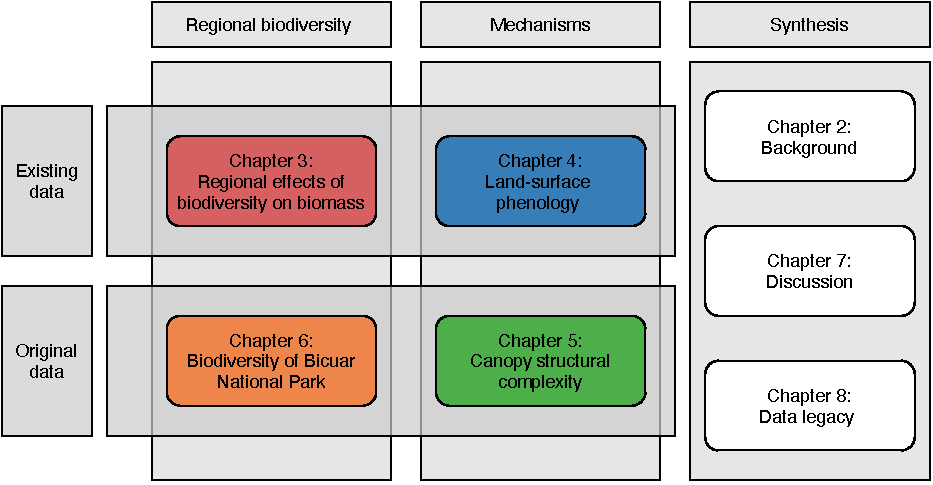
\includegraphics[width=\textwidth]{img/thesis_struc}
	\caption[Thesis structure and data usage.]{The structure of this thesis, showing the thematic focus and data usage in each chapter. Coloured boxes refer to similar colours in \autoref{intro:thesis_map}, which shows the spatial scales of each core chapter.}
	\label{intro:thesis_struc}
\end{figure}

\begin{figure}[p]
	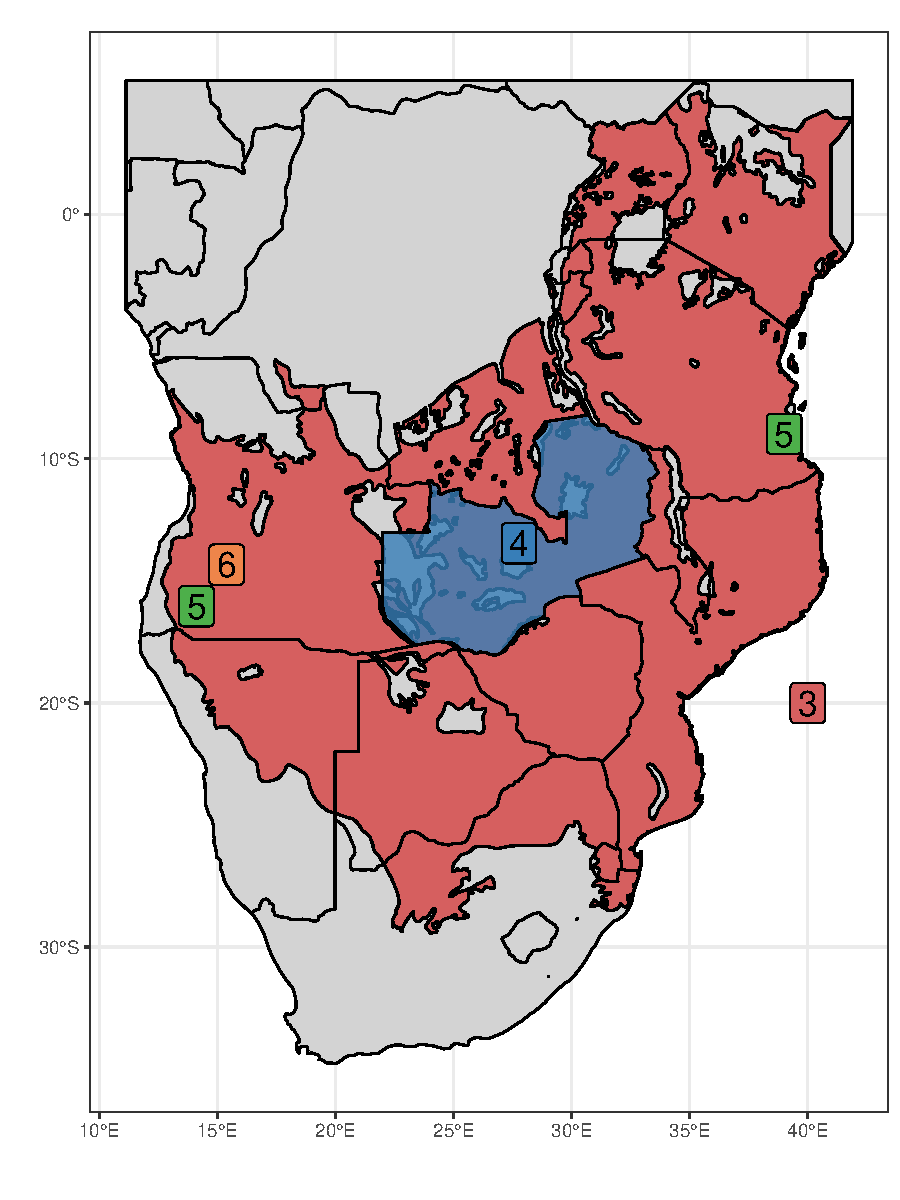
\includegraphics[width=0.8\textwidth]{img/thesis_map}
	\caption[Map of thesis study locations]{The spatial scales of the four core chapters in this thesis. Labels refer to chapter numbers: Chapter 3: The effects of biodiversity on above-ground woody biomass across southern African woodlands. The extent of southern African woodlands is defined by the SEOSAW working region, described in further detail in \autoref{intro:seosaw_plots}. Chapter 4: Effects of tree diversity and composition on land-surface phenology across Zambia. Chapter 5: Biodiversity and canopy structural complexity in Bicuar National Park, Angola (west), and Mtarure Forest Reserve, Tanzania (east). Chapter 6: Woodland composition and structure in Bicuar National Park, Angola.}
	\label{intro:thesis_map}
\end{figure}

\subsection{Chapter 2: Background: The ecology of structure and function in southern African woodlands}
\label{intro:ssec:chp2}

In this chapter, I summarise the literature underpinning the thesis, focussing on two key themes: 1) biodiversity-ecosystem function theory, previous studies and latest developments, and 2) the ecology of tropical savannas, their biogeography within southern Africa, and drivers of structure and function.

\subsection{Chapter 3: A regional assessment of the biodiversity-ecosystem function relationship in southern African woodlands}
\label{intro:ssec:chp3}

Here, I explore whether the positive biodiversity effects on ecosystem function observed in wet tropical and temperate forested ecosystems extends to the mesic savannas of southern Africa. The biodiversity-ecosystem function relationship has been observed to various extents in many experimental and natural systems \citep{Tilman2014, Plas2019}, but low species richness, disturbance by fire and herbivory, and variation in climate might obscure or negate such a relationship in southern Africa. Using existing plot data from the SEOSAW database (\autoref{intro:sssec:seosaw}), I test the interactive effects of: climate, resource availability, disturbance by fire, tree floristic diversity, and woodland structural diversity on woody biomass as a measure of ecosystem function.

\subsection{Chapter 4: Tree diversity and compositional effects on land-surface phenology in deciduous Zambian woodlands}
\label{intro:ssec:chp4}

In this chapter, I test whether species composition and diversity metrics can explain some of the remaining variation in patterns of land-surface phenology in deciduous tropical savannas. The seasonal patterns of foliage growth in deciduous woodlands largely define their gross primary productivity \citep{Penuelas2009}, a key measure of ecosystem function. The pervasive pre-rain green-up observed in deciduous tropical woodlands across southern Africa \citep{Ryan2016} has important consequences for carbon cycling and ecosystem structure \citep{Xia2015}. Climate adequately explains phenological variation across continental spatial scales, but at local scales biotic effects are hypothesised to be more important. I used plot data from the Zambian Integrated Land Use Assessment, which covers the entirety of the country, paired with remotely-sensed measures of green-ness to specifically test: 1) whether species diversity has an observable effect on pre-rain green-up of woodlands, 2) whether species diversity affects growing season length, and 3) whether models of gross primary productivity in deciduous tropical savannas would benefit from the inclusion of higher resolution species compositional data.

\subsection{Chapter 5: Canopy structural complexity as a mechanism for biodiversity effects on productivity}
\label{intro:ssec:chp5}

Canopy packing and the spatial relations among tree canopies is a hypothesised vector of niche complementarity driving positive biodiversity effects on productivity in wooded ecosystems \citep{Jucker2015, Oehri2020}. \citet{Frost1996} describes miombo woodland trees as maintaining high functional diversity, with wide variation in life-history strategies and growth forms among coexisting species. In this chapter I conduct the first assessment of tree canopy structure in southern African woodlands, at two sites in southern Africa, to investigate: 1) the effects of neighbourhood tree species diversity on observed canopy structural complexity, 2) the role of disturbance and spatial distribution of tree stems in driving canopy complexity, and 3), the consequences of variation in tree species diversity for canopy closure and woody encroachment.

\subsection{Chapter 6: Bicuar National Park: a woodland refugia at the extreme western extent of the miombo eco-region}
\label{intro:ssec:chp6}

\citet{White1983} classified miombo woodlands simply as ``dry'' or ``wet'', but this ignores much of the floristic diversity to be found across the miombo eco-region. Understanding the breadth of woodland formations present across southern Africa not only provides vital information for the Dynamic Global Vegetation Models which form the foundation of models of the global carbon cycle \citep{Conradi2020}, but also raises awareness of the conservation value of this diverse phyto-geographic region \citep{Jew2016}. In this chapter, I conduct the first plot-based assessment of the species composition and woodland structure of woodlands in Bicuar National Park, Hu\'{i}la Province, southwest Angola. Specifically, I investigate: 1) the floristic composition of Bicuar National Park compared to other miombo woodlands across the miombo eco-region, 2) the multiple vegetation types found within the Park, and 3) the effects of previous shifting cultivation practices on woodland structure and composition at the boundaries of the Park.

\subsection{Chapter 7: Synthesis: Biodiversity and ecosystem function in southern African woodlands}
\label{intro:ssec:chp7}

Here I discuss the key findings of the thesis. I examine: 1) tree biodiversity effects on ecosystem function as they are mediated by environment and ecological context, 2) tree canopies and physical structure of trees in southern African woodlands as both a product and driver of biodiversity, 3) the mechanisms that may drive observed biodiversity effects in tropical savannas, and 4) the potential consequences of consequences of climate and land use change on woodland ecology as it applies to biodiversity-ecosystem function theory. I conclude by outlining future research that will extend and clarify the findings of the thesis.

\subsection{Chapter 8: Data legacy}
\label{intro:ssec:chp8}

An important outcome of this thesis is the data collected and the research infrastructure that has been cultivated through collaboration with colleagues based in southern Africa. In this chapter I discuss the extended value of the data collected, the steps taken to ensure the data are accessible to others, and provide some ideas for future projects that could use the data to further contribute to our understanding of the carbon dynamics of southern African woodlands.

\section{Data sources and research sites}
\label{intro:sec:sources}

The research presented in this thesis is drawn from three main sources:

\begin{enumerate}
	\item{Existing plot-based data}
	\item{Publicly available geospatial data}
	\item{Original data collected at two research sites within southern Africa}
\end{enumerate}

Background on the various datasets used in the thesis and how each was utilised is discussed below:

\subsection{Existing datasets}
\label{intro:ssec:existing_data}

\subsubsection{SEOSAW}
\label{intro:sssec:seosaw}

Much of the existing data analysed in this thesis, and the locations of field sites used for additional data collection, come from the SEOSAW plot network. SEOSAW - ``a Socio-Ecological Observatory for Southern African Woodlands'' \citep{Ryan2020}, consists of a network of woodland inventory plots across southern Africa (\autoref{intro:seosaw_plots}) and a network of researchers who study the ecology of southern African woodlands. The SEOSAW plot network currently represents the largest plot network in the dry tropics. As of May 2021, it contains 9863 plots, of which 286 are permanent plots where measurement of tree productivity is possible. The plots are of varying size and shape but share a similar methodology in the way woody biomass is estimated, using allometric equations incorporating stem diameter and height measurements with species specific wood density estimates. The plot network spans wide environmental gradients (\autoref{intro:seosaw_space_all}) and floristic types, making it a valuable resource for studying regional variation in tree biodiversity and biomass stocks. During this PhD project I contributed to the development of the SEOSAW database, helping to formalise aspects of the data processing chain, and in developing field data collection methods, as part of SavannaChange, a project funded by the Global Challenges Research Fund (GCRF). Chapter 3 of this thesis uses a subset of 1235 plots from across the region to investigate drivers of aboveground biomass as they relate to species composition and other environmental variables. 

\begin{figure}[p]
	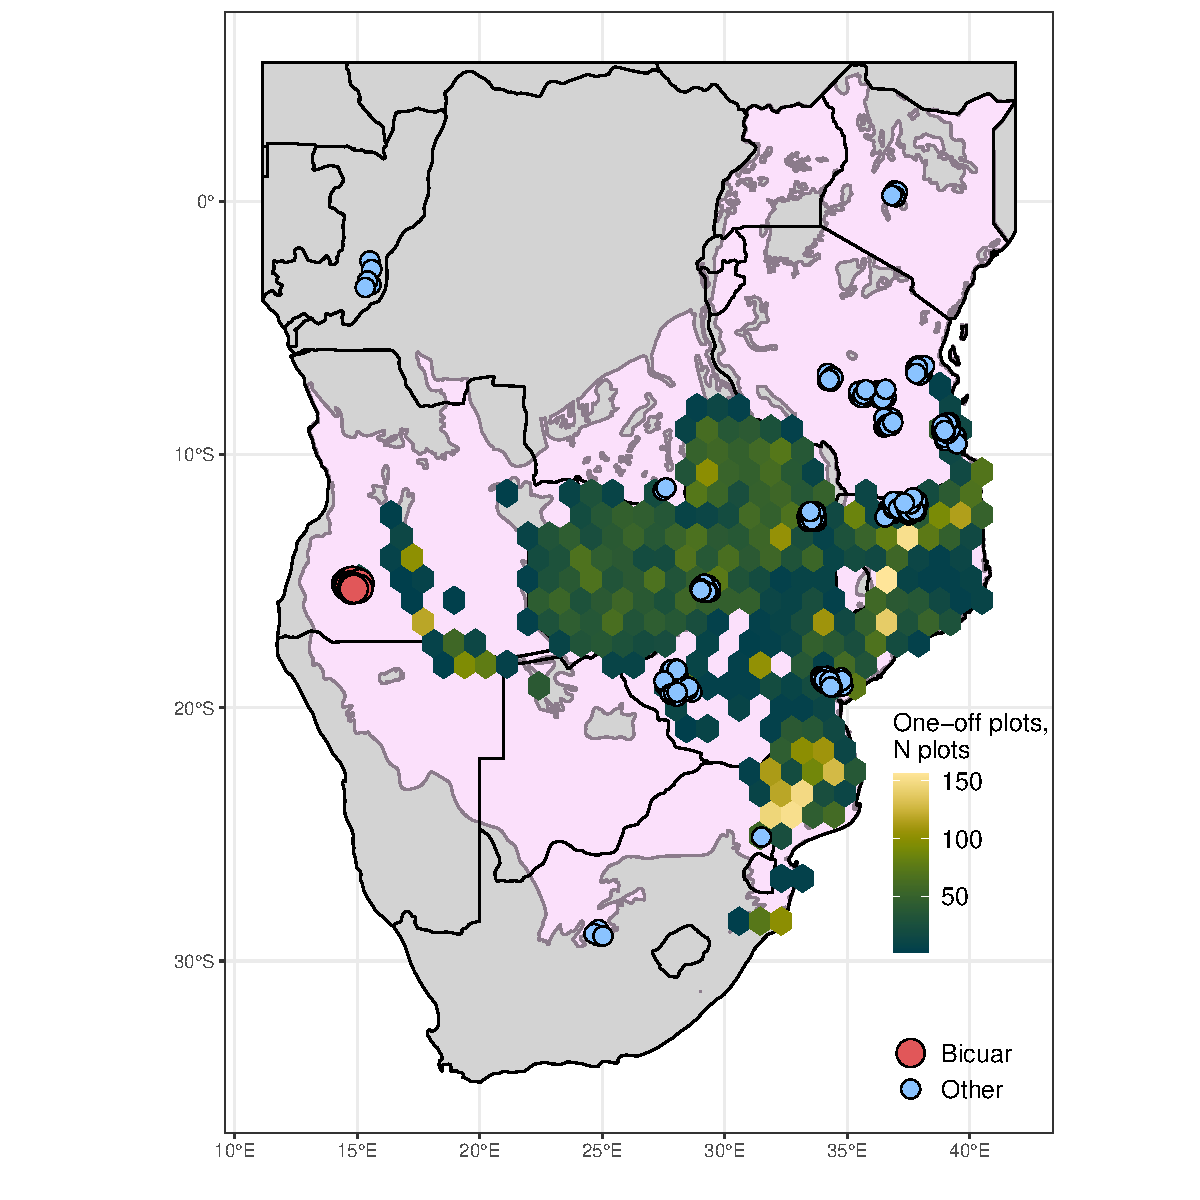
\includegraphics[width=\textwidth]{img/seosaw_plots}
	\caption[Map of SEOSAW plot locations]{The spatial distribution of plots in the SEOSAW network. Blue circles are permanent plots, where individual stems can be matched among censuses. The new permanent plots in Bicuar National Park constructed as part of this thesis are shown as red points. The hexagonal-grid shows the density of one-off plots. The pink shading shows the working region of the SEOSAW network, defined primarily from woodland defined by \citet{White1983} and further adapted to bound the north-eastern and southern boundaries.}
	\label{intro:seosaw_plots}
\end{figure}

\begin{figure}[tb]
	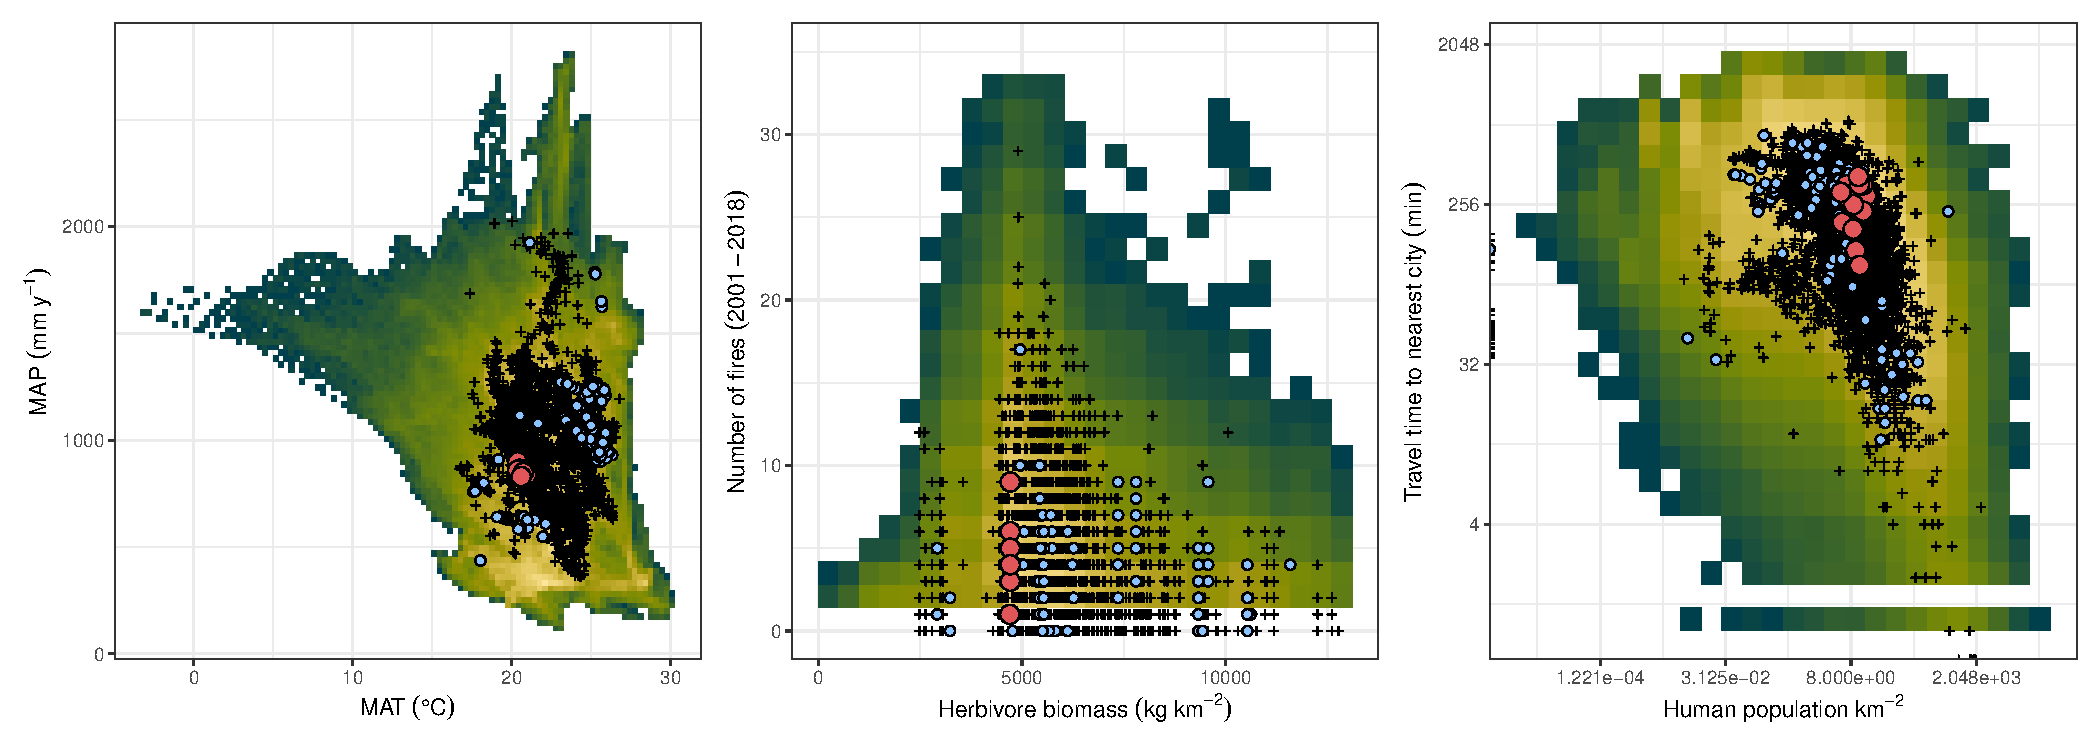
\includegraphics[width=\textwidth]{img/seosaw_space_all}
	\caption[Distribution of SEOSAW plots in environmental space]{SEOSAW plots in various bivariate environmental spaces. Blue circles are permanent plots, where individual stems can be matched among censuses. The permanent plots in Bicuar National Park constructed as part of this thesis are shown as red points. Black crosses show one-off plots. The background of each plot is shaded according to the density of pixels in the SEOSAW working region, as described in \autoref{intro:seosaw_plots}, from blue (low) to yellow (high). From left to right: 1) Climate space, using Mean Annual Temperature (MAT) and Mean Annual Precipitation (MAP), both extracted from the WorldClim dataset gridded at 30" (arc seconds, \textapprox{}900 m at the equator) \citep{Fick2017}. 2) `Disturbance space', using herbivore biomass from \citet{Hempson2017} and fire frequency between 2001 and 2018 from the MODIS burned area product (MCD64A1) \citep{MCD64A1}. 3) `Human influence space', using human population density taken from the WorldPop dataset \citep{Linard2012}, and travel time to nearest city taken from the Malaria Atlas Project \citep{Meijer2018}. Note that both axes for the human influence plot are log transformed.}
	\label{intro:seosaw_space_all}
\end{figure}

\subsubsection{Zambian Integrated Land Use Assessment}
\label{intro:sssec:iluaii}

While The Zambian Integrated Land Use Assessment (ILUAii, \citealt{Mukosha2009}) is included in part within the SEOSAW database, this dataset deserves separate explanation. The ILUAii constitutes that largest single dataset contribution to the SEOSAW database in terms of number of plots (3886/9863) and total area covered (389/1387 ha) as of May 2021 (SEOSAW v2.12). Among other goals related to quantifying the state of natural resources in Zambia, the ILUAii aims to quantify woody biomass and vegetative composition across Zambia. In 2014 a regular grid of one-off plot surveys was conducted across the country, with very few gaps, mostly related to accessibility or lack of natural vegetation. The plot survey collected data on tree species, stem diameter and metadata such as land tenure and human resource usage. Chapter 4 of this thesis uses plot data contributed to the SEOSAW database from the ILUAii to investigate the role of tree species composition and diversity in driving land surface phenology. 

\subsubsection{Climate databases: WorldClim, IMERG}
\label{intro:sssec:clim}

I used multiple climate databases to account for variation in climate, which affects biodiversity, ecosystem function and the interaction between biodiversity and ecosystem function. WorldClim provides up to 30" (\textapprox{}900 m at the equator) monthly climate averages of temperature and precipitation over the period 1970-present \citep{Fick2017}. Additionally, WorldClim provides summarised data known as BioClim, with calculated variables commonly used in ecological science at an annual time-scale such as temperature seasonality and diurnal temperature range. WorldClim provides interpolated climate data utilising weather station data to produce data with known spatial uncertainty, at a higher resolution than similar products such as the CRU TS data \citep{Harris2013}. I used WorldClim throughout the thesis to characterise the climatic context of study sites, but particularly within the Structural Equation Modelling framework of Chapter 3 to understand how environmental covariates mediate biodiversity effects across the southern African subcontinent. IMERG (Integrated Multi-satellitE Retrievals for GPM) \citep{IMERG} provides globally available estimated precipitation daily time series. IMERG has a pixel size of 0.1\textdegree{} (11.1 km at the equator) \citep{IMERG}. I used IMERG precipitation time series in Chapter 4 to quantify the extent of the pre-rain green-up phenomenon in Zambian woodlands. IMERG can be seen as the successor to the well-known TRMM product \citep{Bowman2007}, which no longer provides accurate measurements due to its declining altitude.

\subsubsection{SoilGrids}
\label{intro:sssec:soil}

ISRIC SoilGrids provides modelled estimates of the spatial distribution soil properties, globally, at 250 m resolution \citep{Hengl2017}. SoilGrids incorporates over 230,000 soil profile observations from the WoSIS database \citep{Batjes2017} along with various environmental covariates to estimate soil properties where ground measurements are sparse. I used variables related to soil texture and soil nutrient content such as cation exchange capacity, sand content, and available organic nitrogen, to understand the effect of resource availability on the strength of biodiversity effects on woody biomass across southern African woodlands, in Chapter 3 of this thesis. While the modelled nature of the SoilGrids product relies upon interpolation of spatially sporadic ground measurements with other data such as climate and land use and carries uncertainty as a result, this trade-off also produces a consistent data product that can be used to easily compare many plots where conducting ground measurements would be prohibitively expensive.

\subsubsection{MODIS burned area}
\label{intro:sssec:fire}

The MODIS burned area time series product (MCD64A1) \citep{MCD64A1} uses a combination of burn scars and active fire records to estimate instances of fire, overcoming limitations caused by cloud cover. The MODIS burned area product provides estimates of burned area at a resolution of 500 m, classifying pixels as burned or unburned over a monthly time period. I used the MODIS burned area product to quantify plot-level disturbance regime as mean annual fire frequency in Chapter 3 of the thesis. The majority of the plots used in analyses did not have a comprehensive fire history, thus the MODIS burned area product provided a consistent and easily interpretable alternative. To our knowledge there is no comparable remotely-sensed fire product available with the same spatial and temporal coverage as the MODIS burned area product.

\subsubsection{MODIS EVI}
\label{intro:sssec:evi}

The MODIS EVI (Enhanced Vegetation Index) time series product (MOD13Q1) \citep{MOD13Q1} provides 16 day estimates of EVI at 250 m spatial resolution. EVI uses a simple formula using the Near-InfraRed (NIR) and Red spectral bands from MODIS to estimate ``green-ness''. EVI is considered an improvement over the Normalised Differential Vegetation Index (NDVI) in certain ecological contexts as it corrects for diurnal variation in atmospheric conditions and avoids saturation at higher canopy densities \citep{Huete2002}. I used EVI estimates in Chapter 4 to approximate phenological activity of trees across Zambia.

\subsection{New datasets}
\label{intro:ssec:new_data}

\subsubsection{Permanent plots in Bicuar National Park}
\label{intro:sssec:bicuar}

With colleagues from ISCED Hu\'{i}la, I set up 15 permanent 1 ha woodland survey plots in Bicuar National Park, Hu\'{i}la Province, Angola (S15.1\textdegree{}, E14.8\textdegree{}). The plots were situated along a gradient of stem density. These plots aim to encompass the main woodland types found in the park, which is representative of the natural vegetation found in the larger Hu\'{i}la plateau region \citep{Huntley2019}. Chapter 6 characterises the floristic and structural diversity of the permanent plots in Bicuar National Park, with respect to other plots in the wider miombo eco-region.

Forest mosaics and savanna-woodlands are the dominant vegetation type in Angola \citep{White1983}, and are regarded as under threat as the human population increases, particularly surrounding urban areas \citep{Ritchie2018}, putting pressure on woodlands to provide charcoal and timber. Weak policies in the forestry sector and inadequate government oversight has led to deforestation, particularly in the southern and eastern parts of the country, notably inside protected area boundaries \citep{FAO2015, Mendelsohn2019}. While the annual rate of deforestation in Angola was estimated at 0.2\% in 2005, this has since increased following population growth and development of rural infrastructure such as roads since the end of the civil war \citep{Roder2015}, resulting in an estimated 13.7\% of intact forested habitat being lost between 2000 and 2013 \citep{Potapov2017, Hansen2013}. The biota of much of Angola remains understudied \citep{Huntley2019}. While many conservation areas and national parks were created during the Portuguese colonial era, most were abandoned during the civil war period following independence (1975-2002), with some only recently coming back under active government management \citep{Huntley2019, Ministerio2006}.

Bicuar National Park constitutes the largest intact formation of miombo woodlands in the Hu\'{i}la plateau. The Park has been protected to varying extents since 1938, initially as a game reserve and as a National Park from 1964. The Park was originally 790 km\textsuperscript{2}, but was reduced to \textapprox{}675 km\textsuperscript{2} in 1972 following a governmental decree to allow for the expansion of the Capelongo colonial settlement \citep{Mendelsohn2019}. In 2012, the Park boundaries were re-instated with a new fence and park access gates, following multiple decades of largely absent management. Around the mid-1980s the current park main station was occupied by Cuban militia. During this time many species of large herbivore became locally extinct within the Park, including the African buffalo (\textit{Syncerus caffer}), the plains zebra (\textit{Eqqus quagga}), and the blue wildebeest (\textit{Connochaetes taurinus}).

Bicuar National Park lies at \textapprox{}1200 m asl, sitting on wind-blown Kalahari sand deposits which extends across much of the western portion of southern Africa as far north as the Congo basin \citep{Shaw2002}. The soils underlying the Park are identified as arenosols, consisting of mainly sand with some humus and clay \citep{Jones2013, Hartemink2008}. The Park is located at the transition between miombo woodlands found in moister conditions to the north, and \textit{Baikiaea plurijuga} woodlands which occupy the drier region to the south. The miombo woodlands of the Park are dominated by \textit{Brachystegia} spp. and \textit{Julbernardia paniculata}, while the southern drier woodlands are dominated by \textit{Baikiaea plurijuga} and \textit{Burkea africana} \citep{Teixeira1968}. A distinctive catenal system occupies the north and central parts of the Park, with seasonally flooded grasslands and suffrutex shrublands at the base of the shallow valleys (locally known as ``mulolas''), which drain into the Kunene river, and woodlands on the catenal ridges (locally known as ``tundas''). The climate of the Park is highly seasonal, with a warm rainy season from October to April and cooler dry periods over June and July. SASSCAL provides ongoing meteorological monitoring from a weather station located near the Park centre from 2015 (\autoref{intro:bicuar_weather}).

\begin{figure}[tb]
	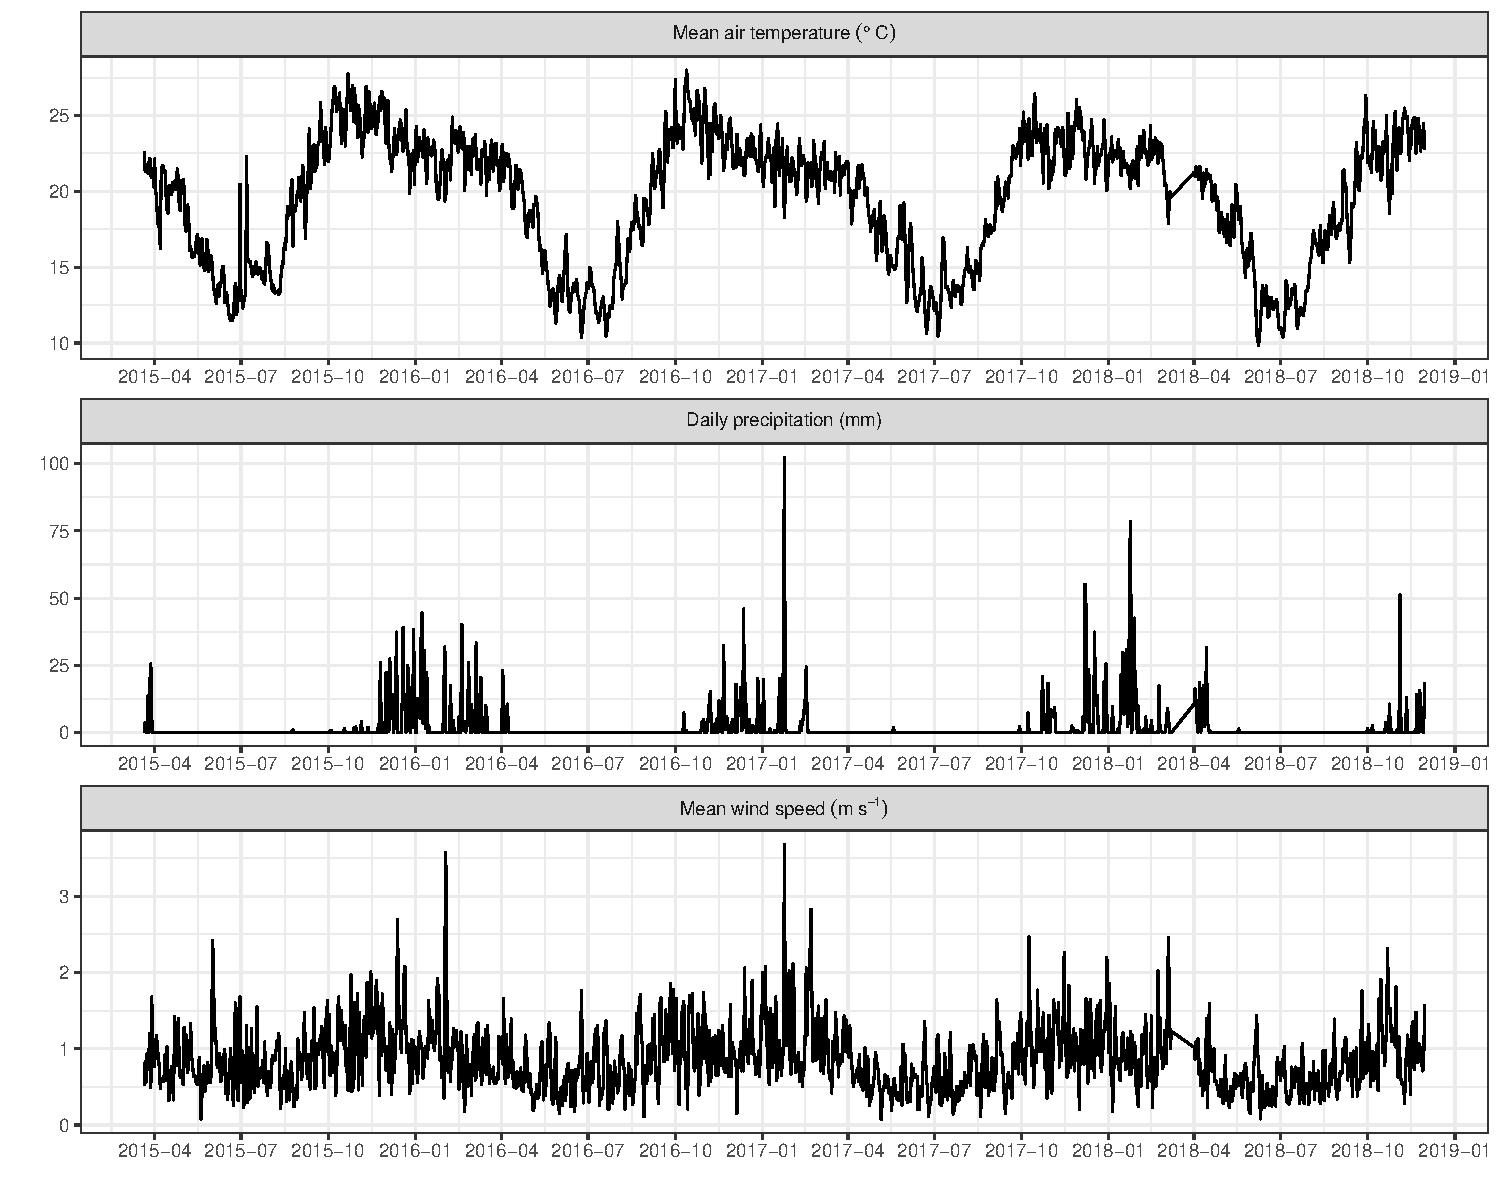
\includegraphics[width=\textwidth]{img/bicuar_weather}
	\caption[Bicuar National Park climate time series]{Data from the SASSCAL weather station located at the main station near the centre of Bicuar National Park. Data are daily aggregates, collected between March 2015 and June 2019.} 
	\label{intro:bicuar_weather}
\end{figure}

The Park currently holds many endemic plant species not found outside the Hu\'{i}la plateau \citep{Huntley2019}, and is home to large herbivores such as elephants (\textit{Loxodonta africana}), giant sable antelope (\textit{Hippotragus niger variani}), and greater kudu (\textit{Tragelaphus strepsiceros}), which travel between Bicuar National Park and the adjacent Mupa National Park to the south. The Park has a number of excavated watering holes to attract large herbivores for observation \citep{Simoes1971}. Other studies indicate populations of other animal species such as the African wild dog (\textit{Lycaon pictus}) \citep{Beja2019, Overton2016} and a number of endemic herptiles \citep{Baptista2019}. Both \citet{Linder2001} and \citet{Droissart2018} identify the Hu\'{i}la plateau as a centre of tropical African botanical endemism, but contemporary studies characterising the exact vegetation composition of the Park are scarce. \citet{Teixeira1968} identified six unique vegetation formations within the Park, including woodlands, shrublands, and grasslands. \citet{Barbosa1970, Chisingui2018} both described the dominance of \textit{Baikiaea}-\textit{Baphia} woodlands particularly in the southern area of the Park. Much of the land cover around the Park has been transformed to agriculture and pasture. Of particular conservation concern is the pattern of land use change in the corridor between Bicuar National Park and Mupa National Park. Further development in this area could fragment the valuable seasonal corridor used by large mammals in the dry season to reach ephemeral water sources \citep{Overton2016}. Additionally, \citet{Catarino2020} described changing patterns of fire across protected areas in Angola, showing that Bicuar National Park is experiencing a rapid increase in fire frequency. They suggest that ingress by humans may be causing the increase in burning, with potential negative consequences for biodiversity and ecosystem integrity. 

\begin{figure}[tb]
	\begin{subfigure}[b]{0.45\linewidth}
		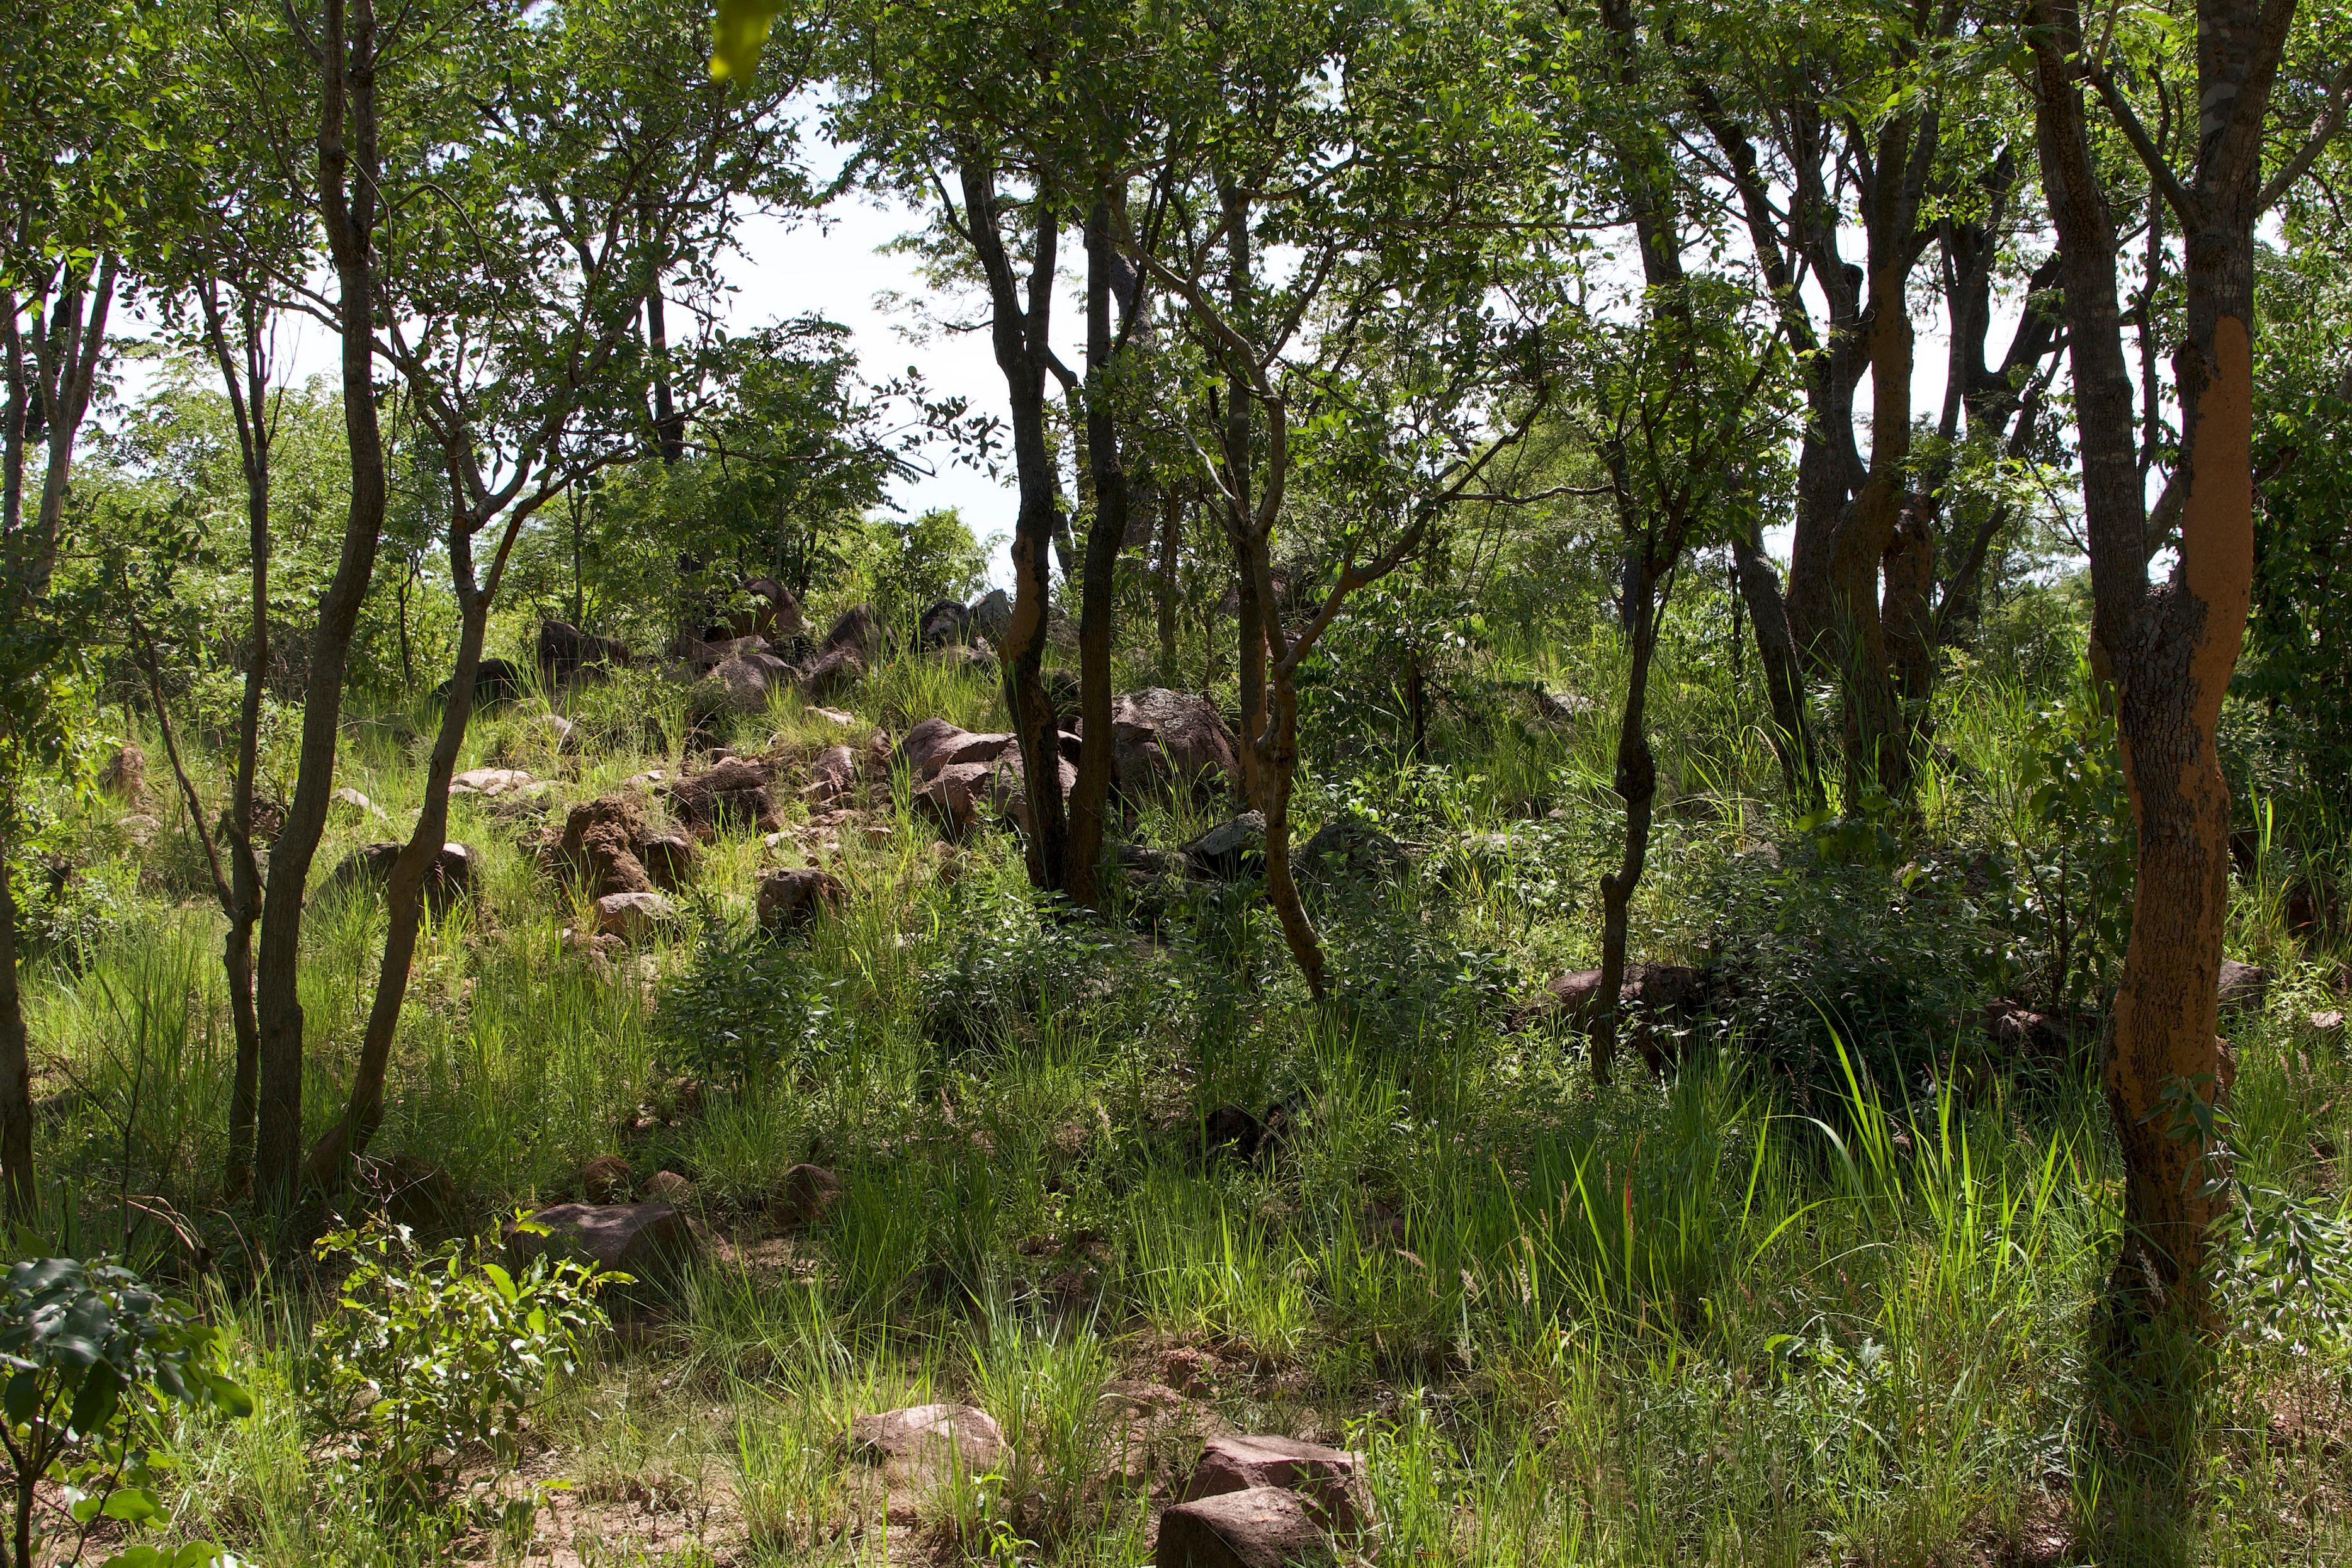
\includegraphics[width=\linewidth]{img/bicuar_photos/julbernardia_crop}
		\caption{}
		\label{intro:julbernardia}
	\end{subfigure}
	\hfill
	\begin{subfigure}[b]{0.45\linewidth}
		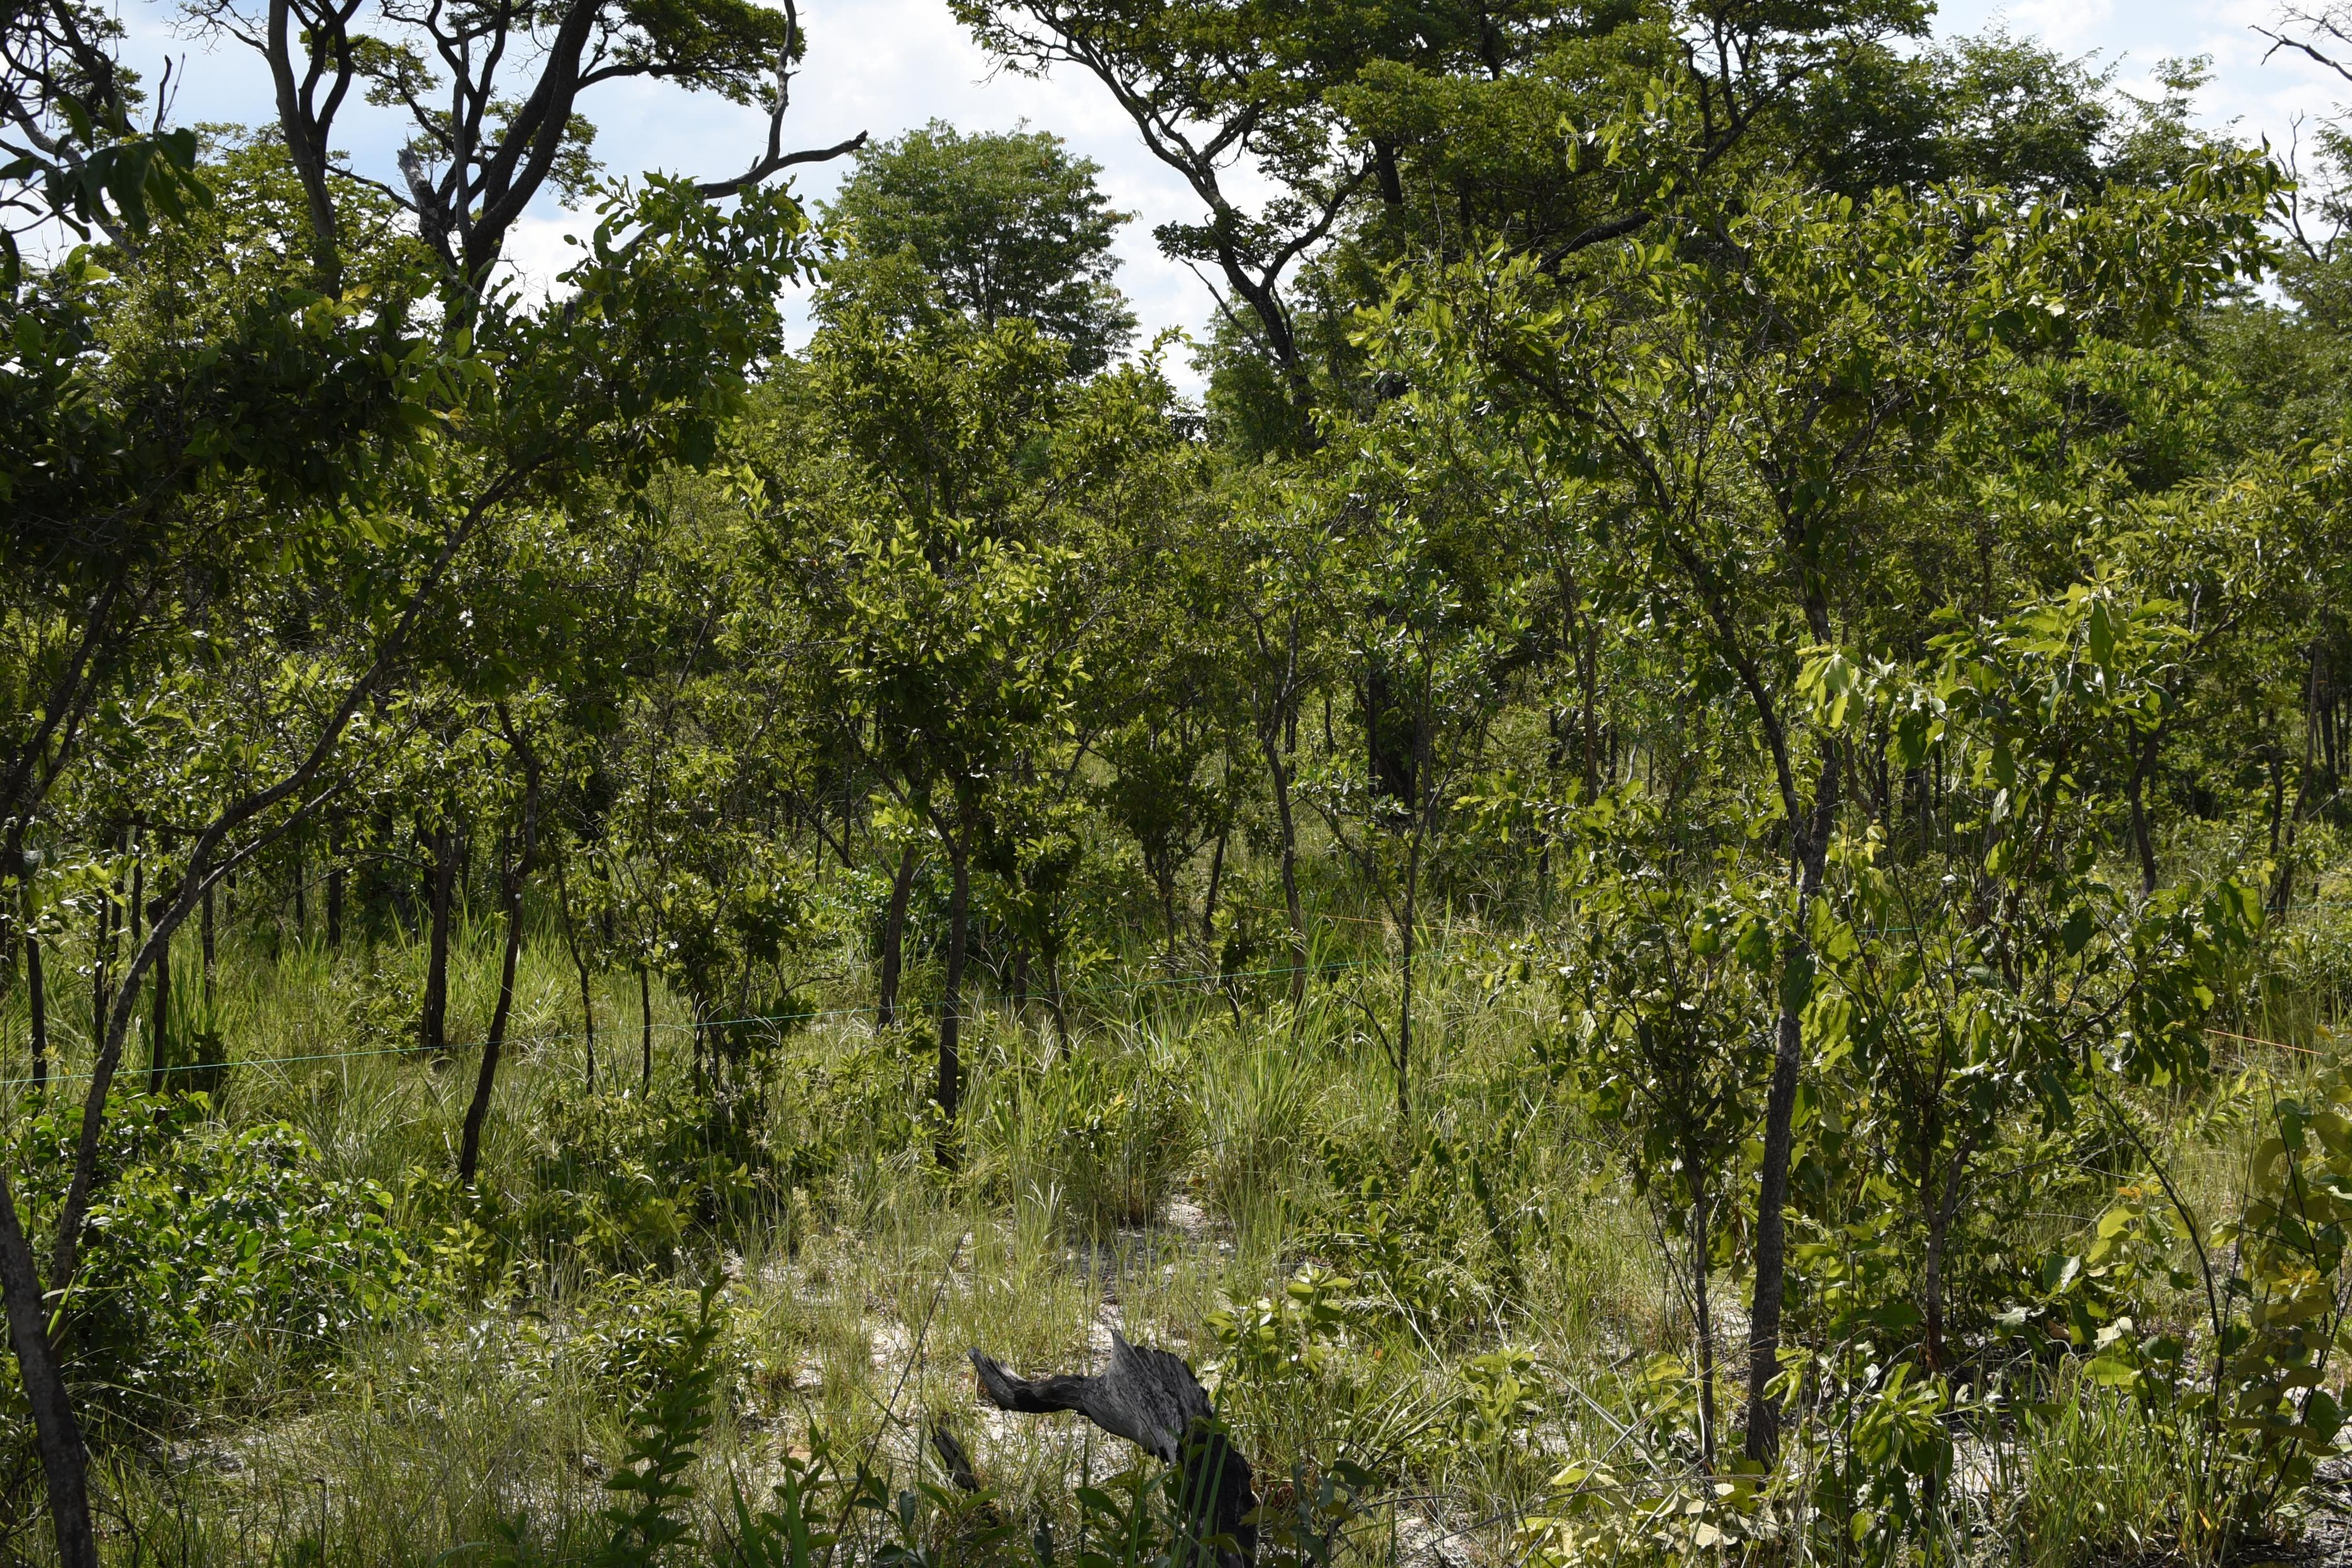
\includegraphics[width=\linewidth]{img/bicuar_photos/burkea_crop}
		\caption{}
		\label{intro:burkea}
	\end{subfigure}
    \vskip\baselineskip
	\begin{subfigure}[b]{0.45\linewidth}
		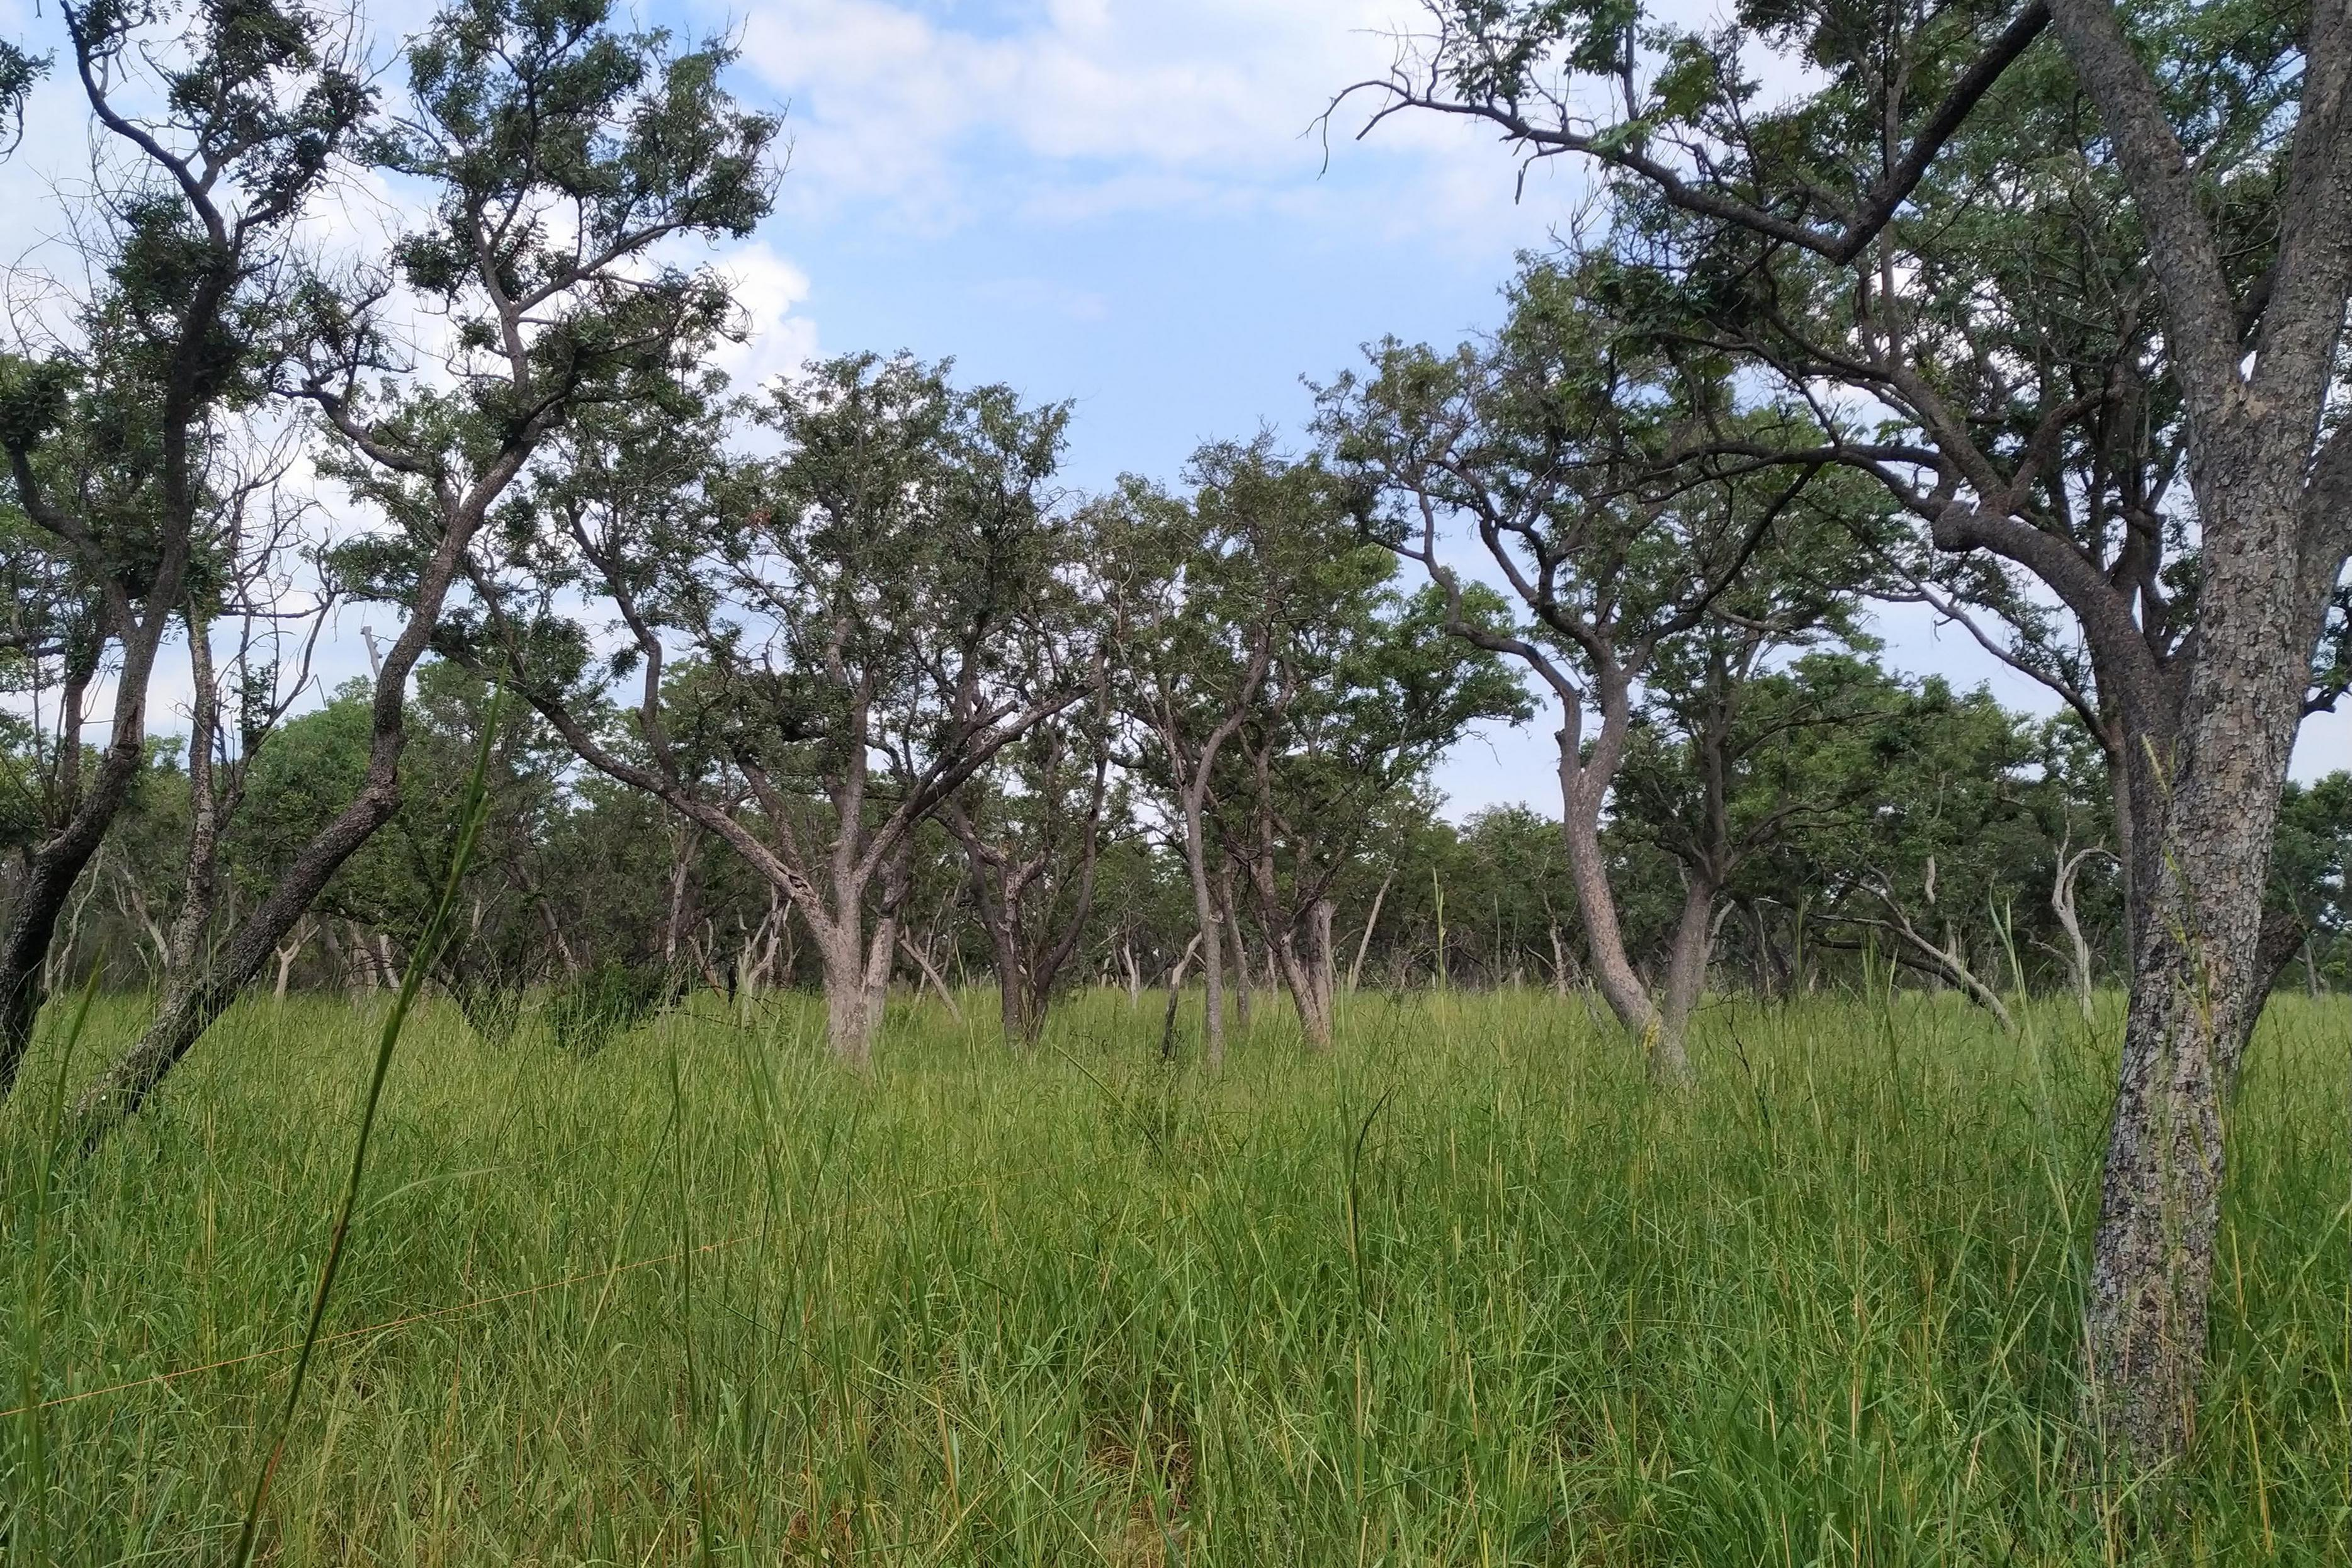
\includegraphics[width=\linewidth]{img/bicuar_photos/baikiaea_crop}
		\caption{}
		\label{intro:baikiaea}
	\end{subfigure}
	\hfill
	\begin{subfigure}[b]{0.45\linewidth}
		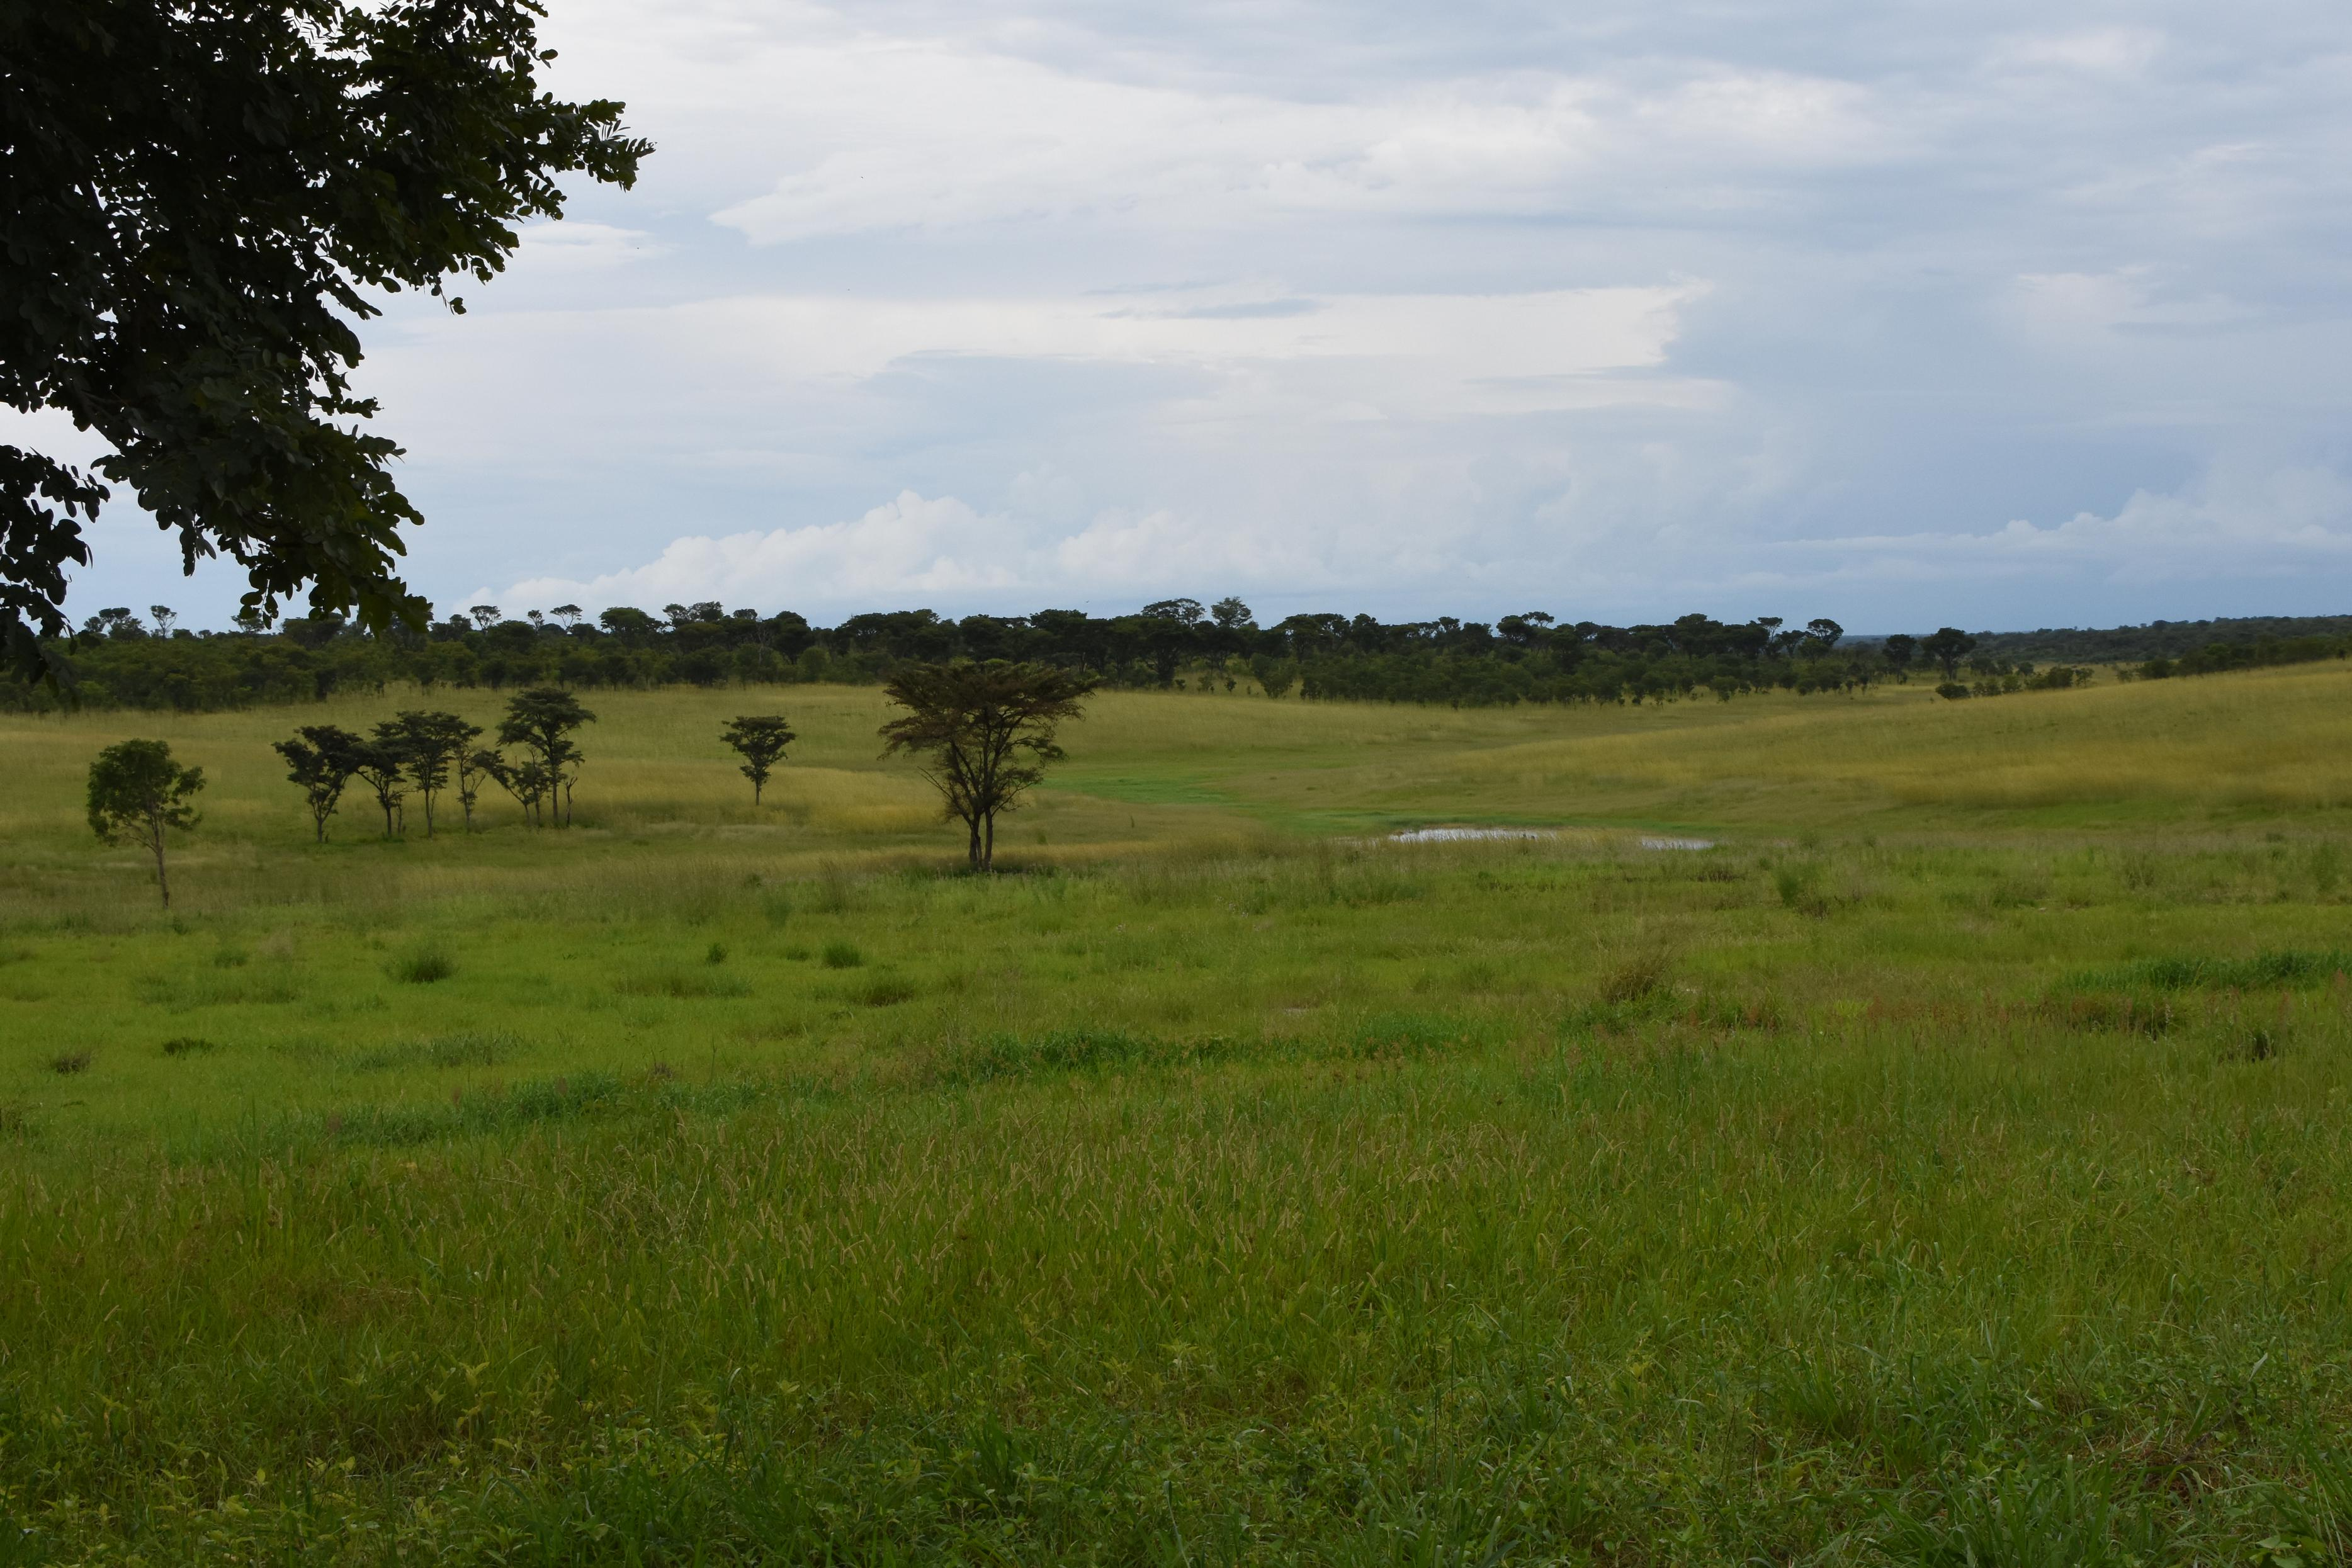
\includegraphics[width=\linewidth]{img/bicuar_photos/mulola_crop}
		\caption{}
		\label{intro:mulola}
	\end{subfigure}
	\caption[Bicuar National Park vegetation type photographs]{The principal vegetation formations seen in Bicuar National Park, southwest Angola. (\subref{intro:julbernardia}) Julbernardia-Brachystegia miombo woodland, (\subref{intro:burkea}) Burkea-Pseudolachnostylis miombo woodland, (\subref{intro:baikiaea}) Baikiaea-Baphia woodland, and (\subref{intro:mulola}) open grassy wetland (``mulola'').}
	\label{intro:bicuar_photos}
\end{figure}

\begin{figure}[tb]
	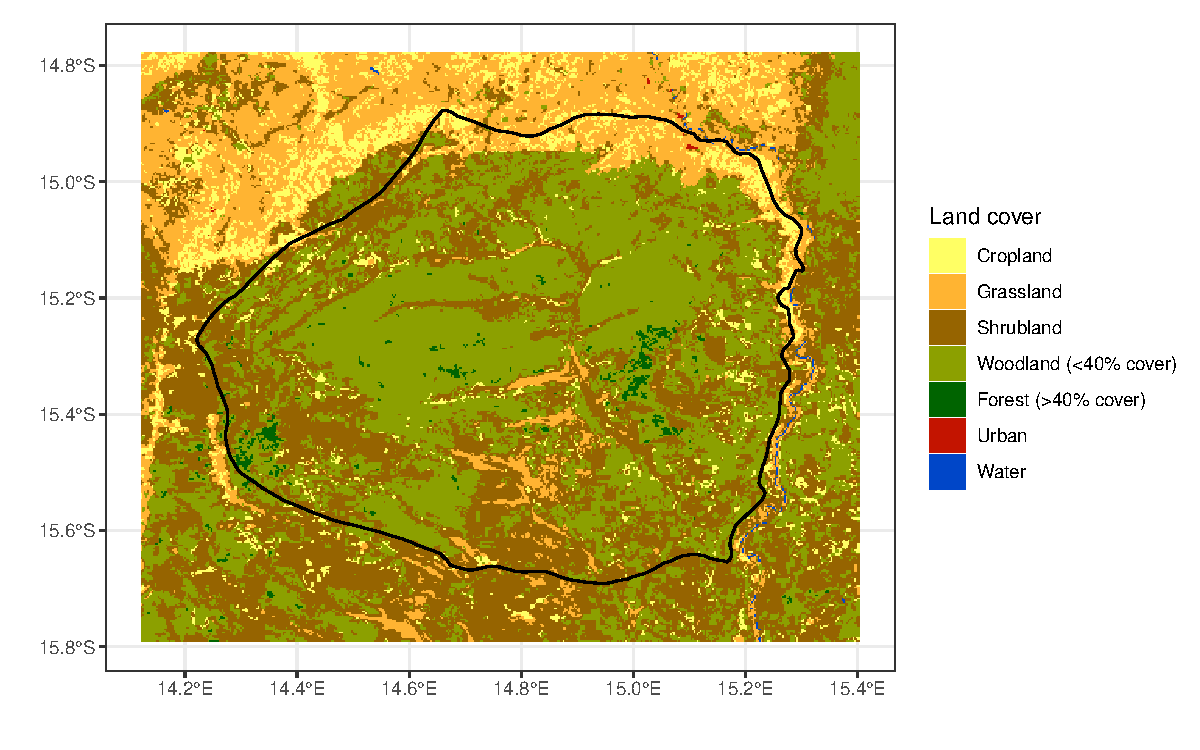
\includegraphics[width=\textwidth]{img/bicuar_land_cover}
	\caption[Bicuar National Park land cover]{Land cover of Bicuar National Park, reclassified from the ESA CCI land cover map (v2.0.7) \citep{ESACCI}. This map highlights the clear deforestation north of the Park, with much land transformed to cropland and grassy pasture. The map also shows the discrepancy between the official park boundary as taken from the World Database on Protected Areas, and the park boundary fence, which is easily seen as a boundary running east-west at approximately S15.0\textdegree{}, E14.8\textdegree{}, with areas of agricultural encroachment beyond the Park boundary fence particularly to northeast of the Park, near the town of Folgares, situated along the Kunene River.}
	\label{intro:bicuar_land_cover}
\end{figure}


\subsubsection{Terrestrial Laser Scanning}
\label{intro:sssec:tls}

Terrestrial laser scanning LiDAR data was collected at two sites which span southern Africa: Bicuar National Park in southwest Angola, and Mtarure Forest Reserve in southeast Tanzania (\autoref{intro:thesis_map}). The two sites both comprise 100x100 m (1 ha) permanent plots in tropical savanna vegetation of varying species composition and stem density. Chapter 5 uses the terrestrial laser scanning data to investigate drivers of canopy structural complexity. Chapter 8 discusses the future research potential of this data. Terrestrial Laser scanning technology provides high-resolution point cloud data that can be analysed in innumerable ways post-hoc to extend its lifespan. Traditional analogue measurements of tree canopy structure are laborious, inaccurate, imprecise and tree-centric, while LiDAR data provides valuable information on inter-tree canopy structure at sub-centimetre precision, albeit at a higher monetary cost, and requiring greater expertise \citep{Xiao2019, Dassot2011}.

\newpage{}
\begingroup
\setstretch{1.0}
\printbibliography[heading=subbibintoc]
\endgroup

\end{refsection}


